\documentclass{beamer}
\usetheme{Boadilla}

\usepackage[backend=biber, style=authoryear, sorting=nty]{biblatex}
\usepackage{amsmath, amssymb, amsthm, mathtools}
\usepackage{bm}
\usepackage{physics}
\usepackage{cleveref}
\usepackage{tikz}
\usetikzlibrary{positioning, backgrounds, arrows.meta}
\usepackage{pgfplots}
\usepackage{booktabs}
\usepackage{caption}
\usepackage{array}
\usepackage{adjustbox}
\usepackage{hyperref}

\pgfplotsset{compat=1.18}


\addbibresource{references.bib}

\setcounter{tocdepth}{2}


\title[Binary Payment Schemes]{Binary Payment Schemes: \\ Moral Hazard and Loss Aversion}
\subtitle{\cite{Herweg2010} \\ Experimental Design}
\author[Theo Osterhaus]{Theo Osterhaus, 7443693}
\date[June 2026]{Seminar Market Design and Behaviour, SuSe 2026}
\institute[WiSo Faculty]{Faculty of Management, Economics and Social Sciences \\ Universität zu Köln}

\begin{document}

\frame{\titlepage}

\begin{frame}{Outline}
    \tableofcontents
\end{frame}

\section{Motivation}

\begin{frame}{Summary: Why Binary Schemes?}
    \begin{itemize}
        \item \textbf{Classical Contract Theory} \parencite{Holmstroem1979}: Optimal contracts should be \textbf{complex}, exploiting all available information.
        \item \textbf{Observation:} Real-world contracts are often remarkably \textbf{simple} (e.g., binary bonus schemes, flat wages).
    \end{itemize}

    \medskip
    
    \textcite{Herweg2010} address this puzzle by introducing \textbf{expectation-based loss aversion} into the standard principal-agent model with moral hazard, building on \textcite{koszegi2007}.
    They identify a trade-off of two opposing effects of adding wage levels:
        
        \medskip
        
        \begin{enumerate}
            \item \textbf{Incentive Gain:} More wage levels (complexity) provide better incentives.
            \item \textbf{Loss Aversion Cost:}  Every additional wage level creates more possible unfavourable comparisons, raising expected psychological costs.
        \end{enumerate}
    \end{frame}
    

\begin{frame}{From Theory to Experiment: Research Question}

    \begin{block}{Motivation: Why Binary Schemes?}
        The central theoretical prediction by \textcite{Herweg2010} that \textbf{binary payment schemes are optimal} has not yet been directly tested empirically.
    \end{block}

    \vspace{0.4cm}
    
    \begin{itemize}
        \item[] \Large \textit{Do binary bonus contracts increase effort beyond multi-level contracts, and is this effect driven by agents' expectation-based loss aversion?}
    \end{itemize}
 
\end{frame}

\section{Related Literature}

\begin{frame}{Related Empirical Literature}

    \begin{itemize}
        \item \textbf{\textcite{Abeler2011}:} Conducted a laboratory experiment showing that expectation-based reference points directly drive workers' effort provision. 
        \item \textcite{Abeler2011} prove the existence of expectation-based reference points in effort provision; my experiment \textbf{explicitly tests the \textit{contractual solution} (Binary vs. Multi-level)} proposed by \textcite{Herweg2010}.

        \medskip
        
        \item Labour Supply (Cab Drivers): \textbf{\textcite{Crawford2011}} shows that a model with expectation-based targets significantly outperforms the neoclassical benchmark in predicting cab drivers' effort.
    \end{itemize}

\end{frame}


\section{Experiment Design}

\begin{frame}{Hypotheses}

    The hypotheses are derived directly from the theoretical predictions in \textcite{Herweg2010} and the expectation-based reference-point model of \textcite{koszegi2007}.

    \vspace{0.3cm}

    \begin{enumerate}
        \item \textbf{H1 (Main Effect Contract):} Effort under the binary contract is greater than or equal to effort under the multi-level contract.
        \begin{itemize}
            \item[\color{gray}\footnotesize$\rightarrow$] \footnotesize\color{gray} \textit{Mechanism: Binary contracts minimize the expected sensation of loss.}
        \end{itemize}
        
        \vspace{0.2cm}
        
        \item \textbf{H2 (Main Effect Reference Point):} A higher reference point leads to higher effort within a given contract type.
        \begin{itemize}
            \item[\color{gray}\footnotesize$\rightarrow$] \footnotesize\color{gray} \textit{Mechanism: Agents adjust their effort to avoid falling short of their expectation-based reference point.}
        \end{itemize}
        
        \vspace{0.2cm}
        
        \item \textbf{H3 (Interaction Effect):} The effort difference between reference-point conditions is \emph{larger} under the multi-level contract than under the binary contract.
        \begin{itemize}
            \item[\color{gray}\footnotesize$\rightarrow$] \footnotesize\color{gray} \textit{This is the central finding of our design. The interaction term ($\beta_3 < 0$).}
        \end{itemize}
    \end{enumerate}

\end{frame}

\begin{frame}{Sampling Methodology \& Recruitment}

    \begin{itemize}
       
        \item \textbf{Target Population \& Subject Pool:} 
        \begin{itemize}
            \item Undergraduate and graduate students across various disciplines.
            \item Recruitment via the university's standard subject pool system (e.g., ORSEE at the Cologne Laboratory for Economic Research).
        \end{itemize}
        
        \item \textbf{Sample Size ($N$):}
        \begin{itemize}
            \item Total $N = 252$ participants ($63$ per treatment group).
            \item Pre-determined via a priori power analysis ($\alpha = 0.05$, $1-\kappa = 0.80$) to detect a medium effect size \textbf{for pairwise cell comparisons}.
        \end{itemize}
    
        \item \textbf{Randomisation \& Assignment:}
        \begin{itemize}
            \item Pure between-subject design.
            \item Participants are randomly assigned to one of the 4 experimental conditions.
        \end{itemize}
    
        \item \textbf{Incentivise \& Execution:}
        \begin{itemize}
            \item \textit{Performance-based pay} to ensure salient economic incentives.
            \item Base show-up fee (e.g., 2.5€) to minimise selection bias and attrition.
        \end{itemize}
    \end{itemize}

\end{frame}

\begin{frame}{Structure of Experiment}
\framesubtitle{Experimental Flow \& $2 \times 2$ Between-Subject Design}

\centering
\scalebox{0.9}{ % Skalierung auf 0.9 erhöht, da das Layout jetzt platzsparender ist
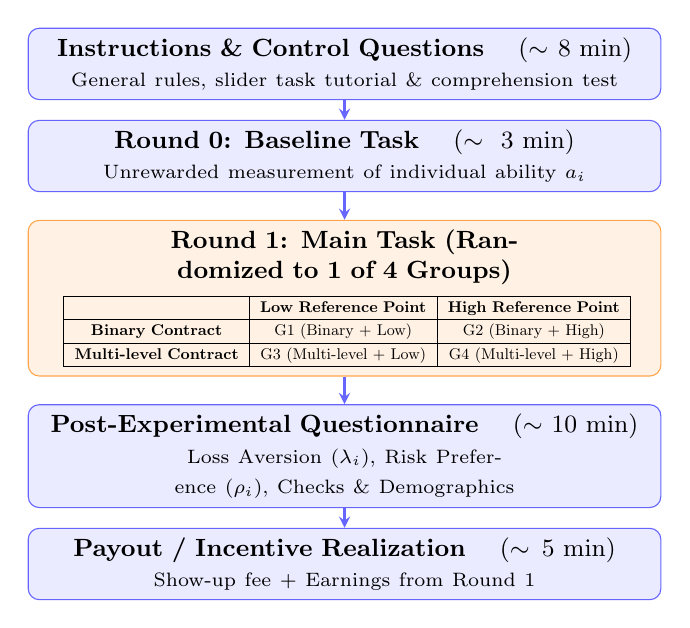
\begin{tikzpicture}[
    station/.style={
        rectangle,
        rounded corners,
        draw=blue!60,
        fill=blue!8,
        text width=7.8cm, % Etwas breiter gemacht, damit alles in eine Zeile passt
        minimum height=0.6cm,
        align=center,
        font=\small
    },
    treatment/.style={
        rectangle,
        rounded corners,
        draw=orange!70,
        fill=orange!10,
        text width=7.8cm,
        minimum height=0.6cm,
        align=center,
        font=\small
    },
    arrow/.style={
        thick,
        ->,
        >=stealth,
        blue!60
    }
]

% Node 1: Instructions
\node[station] (instructions) {
    \textbf{Instructions \& Control Questions} \quad ($\sim 8$ min)\\
    \scriptsize General rules, slider task tutorial \& comprehension test
};

% Node 2: Baseline
\node[station, below=0.25cm of instructions] (baseline) {
    \textbf{Round 0: Baseline Task} \quad ($\sim 3$ min)\\
    \scriptsize Unrewarded measurement of individual ability $a_i$
};

% Node 3: 2x2 Treatment Matrix (Zusammengefasst für mehr Kompaktheit)
\node[treatment, below=0.35cm of baseline] (treatments) {
    \textbf{Round 1: Main Task (Randomized to 1 of 4 Groups)}\\
    \vspace{0.1cm}
    \resizebox{0.95\linewidth}{!}{
        \renewcommand{\arraystretch}{1.2}
        \begin{tabular}{|c|c|c|}
        \hline
        & \textbf{Low Reference Point} & \textbf{High Reference Point} \\
        \hline
        \textbf{Binary Contract}
        & G1 (Binary + Low) & G2 (Binary + High) \\
        \hline
        \textbf{Multi-level Contract}
        & G3 (Multi-level + Low) & G4 (Multi-level + High) \\
        \hline
        \end{tabular}
    }
};

% Node 4: Post-Experimental Questionnaire
\node[station, below=0.35cm of treatments] (survey) {
    \textbf{Post-Experimental Questionnaire} \quad ($\sim 10$ min)\\
    \scriptsize Loss Aversion ($\lambda_i$), Risk Preference ($\rho_i$), Checks \& Demographics
};

% Node 5: Payment
\node[station, below=0.25cm of survey] (payment) {
    \textbf{Payout / Incentive Realization} \quad ($\sim 5$ min)\\
    \scriptsize Show-up fee + Earnings from Round 1
};

% Arrows (Jetzt eine saubere, gerade Linie)
\draw[arrow] (instructions) -- (baseline);
\draw[arrow] (baseline) -- (treatments);
\draw[arrow] (treatments) -- (survey);
\draw[arrow] (survey) -- (payment);

\end{tikzpicture}
}

\end{frame}

\begin{frame}{The Real Effort Task: Slider Task}
\framesubtitle{Experiment Design, by \textcite{GILL2019}}


\centering

\begin{adjustbox}{
    max width=0.98\textwidth,
    max height=0.68\textheight,
    center
}

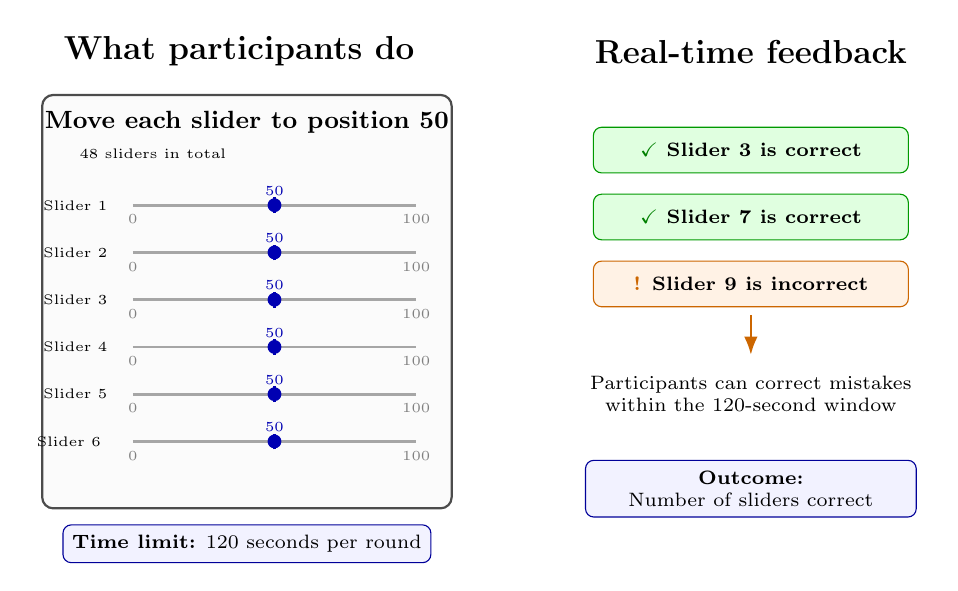
\begin{tikzpicture}[
    >=Latex,
    font=\scriptsize,
    every node/.style={align=center}
]

% =================================================
% LINKES PANEL: AUFGABE
% =================================================

\node[
    font=\large\bfseries
] at (-3.5,1.0)
{What participants do};

% Computer screen
\draw[
    rounded corners=4pt,
    thick,
    draw=black!70,
    fill=gray!3
] (-6.0,-4.8) rectangle (-0.8,0.45);

% Screen title
\node[
    font=\small\bfseries
] at (-3.4,0.1)
{Move each slider to position 50};

\node[
    anchor=west,
    font=\tiny
] at (-5.65,-0.3)
{48 sliders in total};

% Slider rows
\foreach \y/\n in {
    -0.95/1,
    -1.55/2,
    -2.15/3,
    -2.75/4,
    -3.35/5,
    -3.95/6
}{

    % Label
    \node[
        anchor=east,
        font=\tiny
    ] at (-5.05,\y)
    {Slider \n};

    % Track
    \draw[
        line width=1pt,
        draw=gray!70
    ] (-4.85,\y) -- (-1.25,\y);

    % Target marker: position 50
    \draw[
        blue!70!black,
        line width=1pt
    ] (-3.05,\y-0.10) -- (-3.05,\y+0.10);

    % Handle
    \fill[
        blue!70!black
    ] (-3.05,\y) circle (2.5pt);

    % Scale labels
    \node[
        font=\tiny,
        gray
    ] at (-4.85,\y-0.18)
    {0};

    \node[
        font=\tiny,
        blue!70!black
    ] at (-3.05,\y+0.18)
    {50};

    \node[
        font=\tiny,
        gray
    ] at (-1.25,\y-0.18)
    {100};
}

% Time limit
\node[
    draw=blue!60!black,
    fill=blue!5,
    rounded corners=3pt,
    minimum width=4.5cm,
    minimum height=0.48cm,
    font=\scriptsize
] at (-3.4,-5.25)
{\textbf{Time limit:} 120 seconds per round};


% =================================================
% RECHTES PANEL: FEEDBACK
% =================================================

\node[
    font=\large\bfseries
] at (3.0,1.0)
{Real-time feedback};

% Correct feedback
\node[
    draw=green!60!black,
    fill=green!12,
    rounded corners=3pt,
    minimum width=4.0cm,
    minimum height=0.58cm,
    font=\scriptsize\bfseries
] at (3.0,-0.25)
{\textcolor{green!50!black}{\checkmark} Slider 3 is correct};

\node[
    draw=green!60!black,
    fill=green!12,
    rounded corners=3pt,
    minimum width=4.0cm,
    minimum height=0.58cm,
    font=\scriptsize\bfseries
] at (3.0,-1.10)
{\textcolor{green!50!black}{\checkmark} Slider 7 is correct};

% Incorrect feedback
\node[
    draw=orange!80!black,
    fill=orange!10,
    rounded corners=3pt,
    minimum width=4.0cm,
    minimum height=0.58cm,
    font=\scriptsize\bfseries
] at (3.0,-1.95)
{\textcolor{orange!80!black}{!} Slider 9 is incorrect};

% Correction arrow
\draw[
    ->,
    thick,
    orange!80!black
] (3.0,-2.35) -- (3.0,-2.85);

\node[
    font=\scriptsize,
    text width=4.3cm
] at (3.0,-3.35)
{Participants can correct mistakes\\
within the 120-second window};

% Outcome box
\node[
    draw=blue!60!black,
    fill=blue!5,
    rounded corners=3pt,
    minimum width=4.2cm,
    minimum height=0.72cm,
    font=\scriptsize
] at (3.0,-4.55)
{\textbf{Outcome:}\\
Number of sliders correct};

\end{tikzpicture}

\end{adjustbox}

\end{frame}

\begin{frame}{Round 0: Baseline Task}
\framesubtitle{Experiment Design}

    \textbf{Problem:} We need to find a way to introduce a payment structure which is based on individual performance.

    \medskip
    
    \textbf{Solution:} Unpaid slider task to determine individual ability  $a_i$.
    
    \begin{itemize}
      \item We can ensure all participants face the same $80\%$ success probability. \\
      $$\hat{e_i} = 0.8 \times a_i$$
      \item Loss aversion \textit{uniformly} across all groups.
      \item Fair and realistic comparison: Effort differences reflect behavioural response, 
            not ability differences.
    \end{itemize}

\end{frame}

\begin{frame}{Round 1: 2$\times$2 Between-Subject Design}
\framesubtitle{Experiment Design}

\begin{table}[]
\centering
\begin{tabular}{l|c|c}
 & \textbf{Low RP} & \textbf{High RP} \\ \hline
\textbf{Binary Contract} & Group 1 & Group 2 \\ \hline
\textbf{Multi-level Contract} & Group 3 & Group 4 \\
\end{tabular}
\end{table}

\vspace{0.4cm}

\textbf{Contract Structures:}
\begin{itemize}
    \item Binary: $w \in \{w_l, w_h\} = \{2\text{€}, 10\text{€}\}$
    \item Multi-level: $w \in \{w_l, w_m, w_h\} = \{2\text{€}, 6\text{€}, 10\text{€}\}$
\end{itemize}

\vspace{0.3cm}
\centering
\textbf{$N = 252$ (63 per cell), pure between-subject.}

\end{frame}

\begin{frame}{Reference Point Manipulation (Abeler et al. 2011)}
\framesubtitle{Experiment Design}

\textbf{Payout mechanism:} After the slider task, a \textbf{50/50 coin toss} 
determines which payment counts:
\begin{itemize}
    \item \textbf{Heads:} Performance payment (Binary or Multi-level contract)
    \item \textbf{Tails:} Fixed payment $F$
\end{itemize}

\vspace{0.3cm}

\begin{columns}[T]
\column{0.5\textwidth}
\textbf{\textcolor{red}{Low RP:}} $F_{Low} = 4\text{€}$
\column{0.5\textwidth}
\textbf{\textcolor{green!50!black}{High RP:}} $F_{High} = 8\text{€}$
\end{columns}

\vspace{0.4cm}

\begin{exampleblock}{Why this isolates the reference point}
The marginal incentive to exert effort (conditional on the performance branch) is \textbf{identical} across conditions. Only the reference point shifts, via $F$, \textbf{not} via the 
probability.
\end{exampleblock}

\end{frame}

\begin{frame}{Payment Structure}
\framesubtitle{Experiment Design}

    % ---------- PART A: Performance branch (contract type) ----------
    \begin{columns}[T,onlytextwidth]

    \begin{column}{0.48\textwidth}
    \centering
    \textbf{Groups 1 \& 2: Binary Scheme}
    \begin{tabular}{@{}c c@{}}
    \toprule
    \textbf{Sliders correct} & \textbf{Payment} \\
    \midrule
    \( e_i < 0.8\, a_i \)    & $w_l = 2$  \\
    \( e_i \geq 0.8\, a_i \) & $w_h = 10$ \\
    \bottomrule
    \end{tabular}

    \end{column}

    \begin{column}{0.48\textwidth}
    \centering
    \textbf{Groups 3 \& 4: Multi-Level Scheme}
    \begin{tabular}{@{}c c@{}}
    \toprule
    \textbf{Sliders correct} & \textbf{Payment} \\
    \midrule
    $e_i < 0.5\, a_i$                   & $w_l = 2$  \\
    $0.5\, a_i \leq e_i < 0.8\, a_i$    & $w_m = 6$  \\
    $0.8\, a_i \leq e_i$                & $w_h = 10$ \\
    \bottomrule
    \end{tabular}
    \end{column}

    \end{columns}

    \vspace{0.35cm}


    \centering
    \small
    \textbf{Realisation (identical for all groups):} a fair coin flip decides the payout.
    \smallskip

    \begin{tabular}{@{}c l@{}}
    \textbf{Heads} $(p=0.5)$ & Payout $=$ performance pay $w \in \{w_l,w_m,w_h\}$ \\
    \textbf{Tails}\, $(p=0.5)$ & Payout $=$ fixed amount $F$ \\
    \end{tabular}

    \medskip
    
    \scriptsize
    \textit{Note:} By construction, the multi-level scheme has a (weakly) higher expected
    payoff at benchmark effort; potential confound between contract type and expected pay

\end{frame}

\begin{frame}{Post-Experimental Survey \& Measurement of Key Variables}
\framesubtitle{Experiment Design}

    \begin{itemize}
        \item \textbf{Loss Aversion ($\lambda_i$) [Primary Behavioral Variable]:}
        \begin{itemize}
            \item Incentive-compatible Lottery Choice Task (Gächter et al., 2007)
            \item Elicits individual loss aversion parameter $\lambda_i$ via 6 coin-toss decisions
        \end{itemize}

        \vspace{0.15cm}

        \item \textbf{Risk Preference ($\rho_i$) [Control Variable]:}
        \begin{itemize}
            \item General Risk Attitude (SOEP 0--10 Scale) \& Financial Risk Domain
        \end{itemize}

        \vspace{0.15cm}

        \item \textbf{Demographics \& Controls ($X_i$):}
        \begin{itemize}
            \item Age, Gender, Field of Study, Math / Cognitive Ability Self-Assessment
        \end{itemize}
    \end{itemize}

\end{frame}

\section{Analyses}

\begin{frame}{Data Analysis Plan: Econometric Models}
\framesubtitle{Testing Hypotheses \& Research Questions}

    \textbf{Model 1: 2x2 Factorial Design (Testing H1, H2, H3)}
    
    \vspace{-0.15cm}
    
    $$e_i = \beta_0 + \beta_1 \text{Binary}_i + \beta_2 \text{HighRP}_i + \beta_3 (\text{Binary}_i \times \text{HighRP}_i) + \gamma a_i + \delta X_i + \varepsilon_i$$
   
    \begin{enumerate}
        \item \textbf{H1:} $\beta_1 \geq 0$ \textit{(Binary contract yields equal or greater effort than multi-level)}
        \item \textbf{H2:} $\beta_2 > 0$ \textit{(High reference point strictly increases effort)}
        \item \textbf{H3:} $\beta_3 < 0$ \textit{(Interaction: The High RP effect is smaller under the Binary contract)}
    \end{enumerate}

    \begin{itemize}
        \item (RCT) no need of the individual personality traits of the participants ( $\lambda_i; p_i$)
    \end{itemize}

\end{frame}

\begin{frame}{Data Analysis Plan: Econometric Models}
\framesubtitle{Testing Research Questions}

    \textbf{RQ} Do binary bonus contracts increase effort beyond multi-level contracts, and is this effect driven by agents' expectation-based loss aversion?

    \textbf{Model 2: The Driver of the Effect (Addressing the RQ)}
    \vspace{-0.1cm}
    $$e_i = \alpha_0 + \alpha_1 \text{Binary}_i + \alpha_2 \lambda_i + \alpha_3 (\text{Binary}_i \times \lambda_i) + \delta X_i + \varepsilon_i$$
    \begin{itemize}
        \item $\lambda_i$: Individual degree of loss aversion (measured separately).
        \item $\alpha_3 > 0$ verifies the RQ: The effort-increasing effect of binary contracts is driven by agents with stronger loss aversion. (Tests whether the contract 
    \end{itemize}
    
\end{frame}

\begin{frame}{Discussion: Design Choice: Real-Effort Slider Task}
\framesubtitle{No experiment is perfect}

\textcite{BRUGGEN2007}: "Real Effort" and "Chosen Effort" produce different effect sizes.

\vspace{0.3cm}

\textbf{Our Consistency:}
We focus on the \textbf{Slider-Task} by \textcite{GILL2019}, because,

\begin{enumerate}
  \item \textbf{External Validity:} Realistic work behavior 
        (relevant for practice)
  \item \textcite{Herweg2010} is interested in \emph{real} Decisions based on effort, not stylized choices
  \item \textbf{Mechanism Clarity:} Loss aversion affects actual 
        productivity, not just the psychology of choice.
\end{enumerate}

\vspace{0.3cm}

\textbf{Limitations:}
\begin{itemize}
  \item Ability-Confounder
\end{itemize}

\end{frame}

\begin{frame}{Critical Discussion: Limitations \& Trade-offs}
\framesubtitle{No experiment is perfect}

\footnotesize

    \begin{itemize}
        \item Baseline Task Round 0:
        \begin{itemize}
            \item Economic incentive to exert high effort?
            \item Participants might intentionally slack off in Round 0 to secure an artificially low
        \end{itemize}

        \item Deception and Rational Expectations:
        \begin{itemize}
            \item The lottery avoids deception but may feel artificial compared to real-world peer comparisons.
            \item \textbf{Precedent:} Abeler et al. (2011) use identical logic.
        \end{itemize}

        \item Corner Solutions in Effort Provision:
        \begin{itemize}
            \item Marginal cost of physical effort and fatigue are practically negligible
            \item Is the Bonus of up to $8EUR$ even an incentive to perform?
            \item Is there a use case of a control group (with no payment)?
        \end{itemize}

        \item Disentangling Risk Aversion from Loss Aversion:
        \begin{itemize}
            \item Intermediate wage ($w_m$) provides partial insurance and reduces income variance
            \item Challenge to conclusively prove that the observed divergence in effort is strictly driven by expectation-based loss aversion rather than standard risk aversion
        \end{itemize}
    \end{itemize}



\end{frame}

\section*{Bibliography}
\begin{frame}[allowframebreaks]{Bibliography}
    \printbibliography
\end{frame}
    
\appendix
\section*{Appendix}

\begin{frame}{Appendix: Power Calculations (2x2 Design)}
    \textbf{Objective:} Calculate required sample size using the course formula, accounting for 4 experimental groups.
    
    \vspace{0.2cm}
    \textbf{Formula used:}
    $$ N_{comp} = (t_{1-\kappa} + t_{\frac{\alpha}{2}})^2 \cdot \frac{\sigma^2}{P(1-P)\text{MDE}^2} $$

    \vspace{0.2cm}

    \footnotesize
    \textbf{Parameters for a medium effect:}
    \begin{itemize}
        \item $\alpha = 0.05 \implies t_{\alpha/2} \approx 1.96$
        \item $\kappa = 0.20 \text{ (80\% Power)} \implies t_{1-\kappa} \approx 0.84$
        \item $P = 0.5 \implies P(1-P) = 0.25$ (Maximizes power to minimize required $N$)
        \item $\text{MDE} = 0.5\sigma$ (Medium effect size)
    \end{itemize}

    \vspace{0.2cm}
    \textbf{Results \& 4-Group Application:}
    \begin{itemize}
        \item \textbf{Required $N$ per pairwise comparison:} $\approx 126$ ($63$ per group)
        \item \textbf{Planned Total $N$:} $\mathbf{252}$ ($4 \times 63$ participants)
        \item \textbf{Justification:} By targeting $N=252$ ($63$ per cell), the experiment is fully powered (80\%) not only for main effects, but also for the most demanding \textbf{pairwise cell-to-cell comparisons} to detect an effect size of $\text{MDE} = 0.5\sigma$.
    \end{itemize}
\end{frame}

\begin{frame}{Appendix: Variable and Parameter Definitions}
    \vspace{0.2cm}
    \footnotesize
    \begin{table}[]
        \centering
        \begin{tabular}{@{}llp{5.5cm}@{}} % Definiert Spaltenbreiten
            \hline
            \textbf{Symbol} & \textbf{Name} & \textbf{Definition / Type} \\ \hline
            
            \multicolumn{3}{@{}l}{\textbf{Dependent Variables}} \\ \hline
            $e_i$ & Effort & Measured effort of participant $i$ (e.g., number of solved tasks) \\ 
            $\text{BonusCosts}_i$ & Incentive Costs & Total bonus payout made to participant $i$ (in Experimental Currency Units) \\ \hline
            
            \multicolumn{3}{@{}l}{\textbf{Independent Variables (Main Treatments \& Traits)}} \\ \hline
            $\text{Binary}_i$ & Contract Treatment & Dummy: $1$ if Binary Contract, $0$ if Multi-level Contract \\ 
            $\text{HighRP}_i$ & Reference Point Treatment & Dummy: $1$ if High Reference Point group, $0$ if Low Reference Point group \\ 
            $\lambda_i$ & Loss Aversion & Continuous measure of individual expectation-based loss aversion (elicited separately) \\ \hline
            
            \multicolumn{3}{@{}l}{\textbf{Coefficients \& Controls}} \\ \hline
            $\beta_k, \alpha_k, \theta_k$ & Regression Coefficients & Estimated effects of the respective variables on the dependent variable \\ 
            $X_i$ & Control Variables & Vector of individual characteristics (e.g., age, gender, general risk aversion) \\ 
            $\varepsilon_i$ & Error Term & Unobserved, robust standard errors clustered at the session level \\ \hline
        \end{tabular}
    \end{table}
    
\end{frame}

\begin{frame}{Appendix: between-subject problems}

\textbf{Problems with potential solutions}
    \begin{itemize}
        \item Low Statistical Power: Use multiple Rounds per Person and Covariates
        \item No intra-individual comparison: (RCT) Randomisation ensures causality
    \end{itemize}

\textbf{Why the reference point would be contaminated in the “within” case.}
    \begin{itemize}
        \item The reference point is not the status quo, but rather the rational expectation regarding one’s own wage distribution. So if they did both 
    \end{itemize} 
    
\end{frame}


\end{document}